\documentclass[a4paper]{article}

\usepackage{geometry}
\usepackage[francais]{babel}
\usepackage[utf8]{inputenc}
\usepackage{graphicx}
\usepackage[T1]{fontenc}
\usepackage{listings}
\usepackage{caption}
\usepackage{subcaption}
\usepackage{hyperref}

\title{Projet de Machine Learning - Spaceship Titanic}
\author{Antoine ROUMILHAC \\ Alban RIO \\ Nabil DJELLOUDI \\ Mohammed Yacine BRAHMIA}
\date{Mars 2024}

\newcommand{\illustration}[3]{
    \begin{figure}[h!]
        \centering
        \includegraphics[width=#3]{#1}
        \caption{#2}
    \end{figure}
}

\begin{document}
    \maketitle

    Nom de l'équipe Kaggle : On coule

    \section{Analyse des données}

    \subsection{Répartition passagers transportés / non transportés}

    Dans les données d'entraînement, 4378 des passagers ont été transportés, contre 4315 qui ne l'ont pas été, donc l'ensemble est équilibré. On n'aura donc pas à ajouter de poids lors de la phase d'entraînement.

    \subsection{Valeurs manquantes}

    
    Sur la Figure 1, on peut observer qu'il y a des données manquantes dans l'ensemble d'entraînement, mais qu'elles sont globalement réparties entre les différents passagers.
    On va donc pouvoir remplir les données manquantes en exploitant les relations entre les données.
    
    \illustration{images/Figure 1.png}{Heatmap des données manquantes sur l'ensemble d'entraînement}{6cm}
    \subsection{Variables intéressantes}

    La variable CryoSleep semble être très intéressante à utiliser, car comme présenté sur la figure 2, les personnes ayant pris le CryoSleep n'ont très majoritairement pas été transportées,
    et inversement les personnes ayant pris le CryoSleep ont très majoritairement été transportées.
    
    On peut voir sur la figure 3 que les personnes ayant entre 0 et 12 ans ont été transportées en majorité, 
    tandis que celles ayant entre 18 et 25 ans, et entre 30 et 40 ans, ont été peu moins transportées que la moyenne.
    Il serait donc intéressant d'extraire ces tranches d'âge pour les utiliser pour l'entraînement.
    \illustration{images/Figure 2.png}{Répartition des personnes selon le cryosleep et leur état de transport}{6cm}

    
    La figure 4 montre que la majorité des personnes venant de la planète Europa ont été transportés,
    tandis que la majorité des Terriens n'ont pas été transportés. Il serait donc intéressant d'avoir des
    variables booléennes sécifiant si la personne vient d'Europe, ou de Terre.
    
    \illustration{images/Figure 3.png}{Répartition des personnes selon leur âge et leur état de transport}{6cm}
    
    \illustration{images/Figure 4.png}{Répartition des personnes selon leur planète et leur état de transport}{6cm}
    
    Sur la figure 5, on observe une légère tendance selon la destination des passagers.
    Ceux allant à TRAPPIST-1e ont été majoritairement non transportés, tandis que ceux dont la destination est 55 Cancri e
    ont été majoritairement plus transportés. Idem que pour la planète de départ, il faudrait créer une variable booléenne
    qui est à Vrai si le passager va TRAPPIST-1e, et une autre à Vrai si la personne va à 55 Cancri e.

    \illustration{images/Figure 5.png}{Répartition des personnes selon leur destination et leur état de transport}{6cm}
    
    La figure 6 présente les dépenses des passagers dans le Room Service (en échelle logarithmique sur l'axe des abscisses).
    On peut y voir que ceux n'ayant pas dépensé dans le Room Service ont été très majoritairement transportés.
    A l'inverse, parmi la petite part de passagers ayant dépénsé de l'argent, la majorité n'a pas été transportée.
    La tendance est la même pour les autres postes de dépense.
    Il serait donc intéressant d'avoir une variable booléenne à Vrai si le passager a dépensé de l'argent,
    en complément des variables flottantes de dépenses.

    \illustration{images/Figure 6.png}{Répartition des personnes selon leurs dépenses dans le room service et leur état de transport}{6cm}

    Pour analyser les tendances pour l'identifiant des cabines, on l'a découpé selon les indications du sujet :
    le pont (Deck : de A à G et T), le numéro de cabine, et le côté (Side : S ou P). La figure 7 montre le résultat de ces découpes.

    On peut observer que les passagers sur les ponts B et C ont été majoritairement transportés,
    tandis que les passagers sur les ponts F et E ont été majoritairement non transportés.
    Aussi, les passagers sur le côté S ont été majoritairement non transportés.
    Il serait donc intéressant de transformer ces deux variables en des variables booléennes
    à Vrai si la cabine du passager se trouve sur le pont B, C, F ou E, et si elle se trouve sur le côté S.

    Concernant le numéro de cabine, on peut observer qu'il y a des intervalles de numéros de cabine, dans lesquels 
    les occupants sont soit majoritairement transportés, soit majoritairement non transportés.
    Il serait donc judicieux de transformer cette distribution d'entiers en un ensemble de variables booléennes,
    reflétant dans quel intervalle le numéro de la cabine du passager se trouve.

    \begin{figure}
        \centering
        \begin{subfigure}{.5\textwidth}
            \centering
            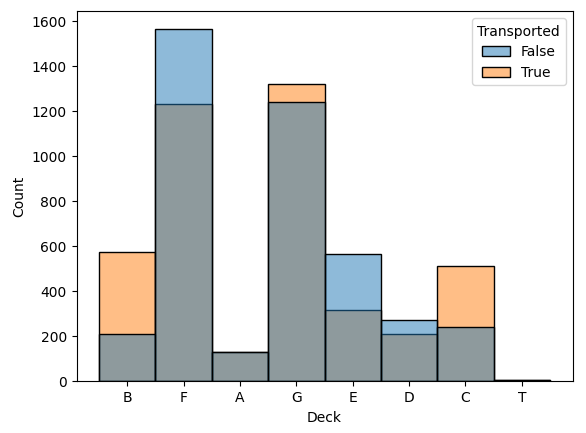
\includegraphics[width=\linewidth]{images/Figure 7-1.png}
            \caption{Pont (Deck)}
        \end{subfigure}%
        \begin{subfigure}{.5\textwidth}
            \centering
            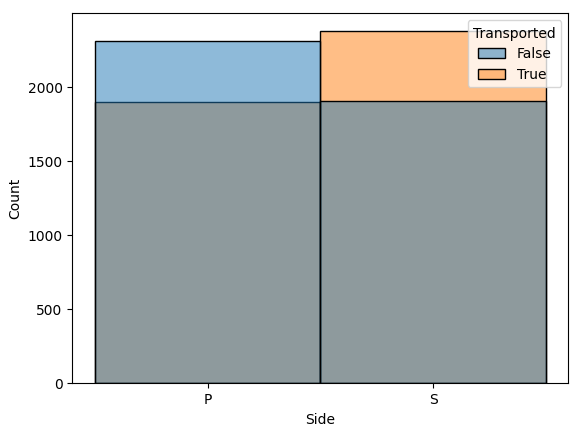
\includegraphics[width=\linewidth]{images/Figure 7-2.png}
            \caption{Côté (Side)}
        \end{subfigure}
        \begin{subfigure}{.5\textwidth}
            \centering
            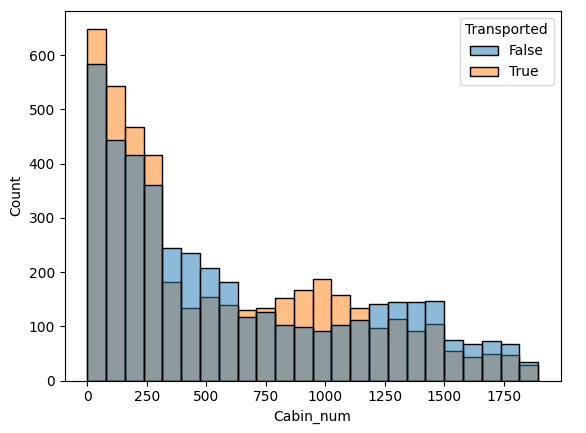
\includegraphics[width=\linewidth]{images/Figure 7-3.png}
            \caption{Numéro de cabine}
        \end{subfigure}
        \caption{Répartition des passagers selon leur cabine}
    \end{figure}

    \section{Prétraitement des données}

    Avant toute chose, on récupère le numéro de groupe de chaque passager, qui est donné par les 4 premiers chiffres
    de l'identifiant de passager (de la forme GGGG\_NN).

    \subsection{Traitement des données manquantes}

    Comme relevé plus haut, il y a de nombreuses données manquantes dans l'ensemble d'entraînement,
    et elles sont réparties entre un grand nombre de passagers différents, ce qui exclut l'élimination
    des lignes avec des valeurs manquantes.

    On doit donc trouver des relations entre les différentes données disponibles.

    Tous les membres d'un même groupe viennent de la même planète. Donc pour les passagers dont la planète d'origine
    est inconnue et dont au moins un autre passager du même groupe a sa planète d'origine connue,
    on peut en déduire la planète d'origine du passager.

    Pour les passagers dont la cabine est manquante, on fait l'hypothèse qu'ils partagent la même cabine qu'un autre
    membre de leur groupe (arbitrairement, le premier membre qu'on trouve dont la cabine n'est pas inconnue).

    Les personnes en CryoSleep ne dépensent pas d'argent (logique), donc on peut supposer que les personnes
    n'ayant pas dépensé d'argent et dont le statut de CryoSleep est inconnu, sont en CryoSleep.

    Pour les passagers qui ne sont pas en CryoSleep et qui n'ont rien dépensé, on peut raisonnablement supposer que ce sont des enfants
    de moins de 12 ans, car aucun d'entre eux n'a dépensé d'argent dans l'ensemble d'entraînement.

    Les passagers ayant toujours un statut de CryoSleep inconnu voient leur variable CryoSleep mise à Faux,
    étant donné que les passagers étant en CryoSleep sont minoritaires sur le vaisseau.

    Idem concernant les VIP, ceux-ci étant très minoritaires dans le vaisseau, on définit la variable VIP lorsqu'elle est manquante à Faux.

    Pour remplir les valeurs manquantes de pont, on utilise le fait que les Terriens sont majoritairement au pont G,
    tandis que les passagers d'Europa sont majoritairement aux ponts B et C (on utilise leur dépense pour trancher, ceux du deck C étant moins dépensiers).
    Les Martiens sont eux majoritairement sur le pont F.

    A l'inverse, pour finir de remplir les valeurs manquantes des planètes d'origine, on utilise le pont sur lequel sont les passagers.
    Les passagers sur les ponts A, B, C et T sont majoritairement d'Europa, ceux sur E, F et G sont majoritairement des Terriens, tandis que
    ceux sur le pont D sont majoritairement des Martiens.

    Pour finir de remplir les planètes d'origine, on utilise la destination des passagers.
    Ceux allant vers TRAPPIST-1e et PSO J318.5-22 sont en effet en grande partie des Terriens.
    Finalement, pour ceux dont la valeur est encore manquante, on les définit comme venant d'Europa,
    étant donné qu'il y a plus de personnes d'Europa que de Martiens.

    Enfin on définit les destinations manquantes comme étant TRAPPIST-1e, et les âges comme étant l'âge médian.

    Au terme de ces traitements, nous n'avons donc plus de valeurs manquantes dans l'ensemble d'entraînement et de test.

    \subsection{Traitement et choix des variables}

    Avant toute chose, on crée également une variable booléenne, nommée $Solo$, qui est à 1 si un passager voyage seul, 0 sinon. 
    On utilise pour cela les numéros de groupe qui sont présents dans le $PassengerId$. En effet, un passager a significativement plus de chance d'être
    transporté s'il est seul que s'il est en groupe, comme montré dans la figure 8.

    \illustration{images/Figure 8.png}{Répartition des passagers selon qu'ils voyagent seuls ou non}{8cm}

    Pour les variables de type nombre flottant concernant les dépenses des passagers, nous avons décidé de toutes les garder, car expérimentalement
    les résultats étaient meilleurs avec, plutôt qu'en utilisant des variables booléennes qui reflètent le fait que le passager a dépensé ou non.
    Toutefois, parce que la majorité des passagers ne dépensent pas, il nous a semblé intéressant de créer la variable booléenne $NoSpending$
    qui est à Vrai si le passager n'a rien dépensé, ainsi que la variable $Expenditure$ qui est la somme de toutes les dépenses du passager.
    On a également décidé de passer ces variables au logarithme, pour réduire l'écart-type et avoir de meilleurs résultats : $depenses_{log} = \log{(1+depenses)}$

    Pour la variable $Age$, et comme noté dans l'analyse statistique, on peut discerner une tendance pour $Transported$ selon la classe d'âge
    des passagers. On crée donc 6 variables booléenne reflétant l'appartenance à une classe d'âge pour chaque passager : \textit{0-12}, \textit{12-18}, \textit{18-25}, 
    \textit{25-30}, \textit{30-50} et \textit{50}.
    Chaque variable est à 1 si le passager fait partie de cette classe d'âge, 0 sinon. 

    On fait une manipulation similaire concernant le numéro de cabine, en les divisant en groupes de largeur 300, c'est-à-dire en ayant une variable
    à 1 si le numéro est entre 0 et 299, 0 sinon, une autre variable à 1 si le numéro est entre 300 et 599, 0 sinon, ... , et enfin une variable à 1 si le numéro 
    est supérieur à 1800, 0 sinon. Elles sont nommées {\it Cabin\_region1}, {\it Cabin\_region2}, etc. jusqu'à {\it Cabin\_region7}.

    Ensuite on encode les variables $Side$, $Deck$, $HomePlanet$ et $Destination$, en les remplaçant par un nombre de variables booléennes égal au nombre
    de valeurs différentes de chaque variable, qui sont à 1 ou 0 selon que la variable d'origine avait la valeur correspondant à chaque nouvelle variable.
    Cela suit le principe du One-Hot Encoding. Il est nécessaire de l'utiliser car les algorithmes que nous avons utilisé ne supportent pour la plupart pas
    la présence de variables non numériques dans l'ensemble d'entraînement.

    On a ainsi terminé le traitement des variables, on peut désormais supprimer les variables inutiles. On supprime tout d'abord les variables qui prennent une valeur
    unique par passager : $PassengerId$ et $Name$.
    Ensuite, on enlève les variables qu'on a transformé au préalable en ensemble de variables booléennes : $Age$ et $Cabin_number$.
    De même pour celles qui ont été encodées : $Side$, $Deck$ $HomePlanet$ et $Destination$.

    Ensuite, on a fait le choix de supprimer deux des variables restantes : $Side_P$, car le vaisseau n'ayant que deux côtés, cette variable est
    redondante par rapport à $Side_S$, et $Deck_T$ car le nombre de passagers sur ce pont est extrêmement faible, et il n'y pas de tendance significative
    donc la garder créerait du bruit.

    Finalement, pour sélectionner les variables booléennes les plus intéressantes de l'ensemble d'entraînement, on a codé une fonction qui calcule pour chaque variable
    entière un score. Plus ce score est élevé, plus la variable voit une grande différence entre le nombre de passagers qui ont cette variable à 1 (soit True) et qui ont été transportés,
    et le nombre de passagers dont la valeur est aussi à 1 (soit True) et qui n'ont pas été transportés, et ce relativement à la taille de l'échantillon.
    Nous avons essayé plusieurs formules pour calculer ce score, et les meilleurs résultats ont été obtenus avec celle-ci : 
    $$ score_{var} = \frac{abs(|Tdataset_{Transported=True \land var=True}| - |Tdataset_{Transported=False \land var=True}|)}{|Tdataset|} $$
    où $Tdataset$ correspond à l'ensemble d'entraînement, et $abs$ à la fonction valeur absolue.
    Diviser par le nombre total de passagers permet d'éviter qu'une variable qui est à 1 pour très peu de passagers ne soit gardée,
    évitant ainsi un sur-entraînement, qui pourrait être dû à du bruit ou à un manque de données dans l'ensemble d'entraînement.

    Le nombre optimal de variables à sélectionner peut être légèrement différent selon l'algorithme d'apprentissage utilisé, 
    mais nous garderons ici 22 variables, ce nombre nous donnant les meilleurs résultats avec l'algorithme que nous avons choisi au final. 

    \section{Méthodes et paramètres}

    \subsection{Sélection des hyperparamètres}

    Pour sélectionner les meilleurs hyperparamètres, nous avons utilisé deux fonctions de la librarie scikit-learn : {\it GridSearchCV} et {\it RandomizedSearchCV}.
    Les deux fonctions sont similaires, elles testent les performances des modèles avec différentes combinaisons d'hyperparamètres d'après un ensemble de valeurs d'hyperparamètres
    qui leur sont données, la différence étant que {\it GridSearchCV} teste toutes les combinaisons possibles, tandis que
    {\it RandomizedSearchCV} n'en teste qu'un nombre prédéterminé, permettant d'accélérer les tests.

    \subsection{Méthodes à base de forêts}

    Après avoir regardé les solutions données par les autres participants à la compétition, et en raison du grand nombre de variables booléennes que nous avons dans notre
    ensemble d'entraînement, nous avons commencé par utiliser des algorithmes à base de forêts.

    \subsubsection{RandomForestClassifier}

    Tout d'abord, nous avons utilisé l'algorithme RandomForestClassifier, fourni par la bibliothèque scikit-learn.
    C'est un algorithme basé sur une forêt d'arbres de décision, ces derniers étant entraînés sur des sous-ensembles aléatoires de l'ensemble de départ.
    Les hyperparamètres que nous avons testés pour cet algorithme sont {\it n\_estimators}, qui détermine le nombre d'arbres d'arbres dans la forêt,
    et {\it max\_depth}, qui détermine la profondeur maximale des arbres.

    \subsubsection{GradientBoostingClassifier}

    Nous avons ensuite essayé l'algorithme {\it GradientBoostingClassifier} et sa variante {\it HistGradientBoostingClassifier}, également de la bibliothèque scikit-learn.
    Comme leur nom l'indique, ils utilisent la technique du Gradient Boosting pour parvenir à leurs résultats. 
    D'après le site de scikit-learn \footnote{\url{https://scikit-learn.org/stable/auto_examples/ensemble/plot_forest_hist_grad_boosting_comparison.html}}, les performances de
    ces algorithmes peuvent être meilleures que {\it RandomForestClassifier}.
    Les hyperparamètres que nous avons testés pour ces algorithmes sont {\it learning\_rate}, le taux d'apprentissage qui définit l'importance de la contribution de chaque arbre ;
    {\it n\_estimators}, qui correspond au nombre d'étapes de boosting que l'algorithme va réaliser ; et {\it max\_depth} qui correspond à la profondeur maximale de chaque arbre.

    \subsubsection{LGBMClassifier}

    Nous avons également testé un autre algorithme qui est revenu régulièrement dans les solutions des autres participants, qui est LGBMClassifier,
    de la bibliothèque LightGBM. Il s'agit également d'un algorithme de Gradient Boosting, et les auteurs promettent de meilleurs résultats et un temps 
    d'entraînement réduit par rapport aux autres algorithmes de Gradient Boosting.
    Tout comme le principe de l'algorithme, les hyperparamètres sont assez similaires à ceux de {\it GradientBoostingClassifier}. Nous avons donc testé les
    mêmes, à savoir {\it learning\_rate }, {\it n\_estimators} et {\it max\_depth}, et en plus de cela nous avons aussi testé {\it num\_leaves}. Ce dernier définit
    le nombre maximum de feuilles pour chacun des arbres construits par l'algorithme.

    \subsubsection{CatBoostClassifier}

    Enfin, le dernier algorithme basé sur des arbres que nous avons testé est {\it CatBoostClassifier} de la bibliothèque CatBoost.
    Encore une fois, il s'agit d'un algorithme de Gradient Boosting sur des arbres de décision, mais qui promet toutefois 
    de très bonnes performances même avec les paramètres par défaut.
    L'algorithme est en effet capable de calculer lui même le taux d'apprentissage optimal à partir de l'ensemble d'entraînement, permettant de
    réduire le temps passé à tester tous les paramètres. Nous avons toute fois commencé par tester nous mêmes les valeurs 
    de taux d'apprentissage optimales pour confirmer que le calcul réalisé est correct.
    Les hyperparamètres que nous avons testés sont donc {\it learning\_rate}, {\it n\_estimators} et {\it max\_depth}.

    \subsection{Autres algorithmes testés}

    \subsubsection{SVC}

    Nous avons également testé {\it SVC} de scikit-learn, qui est l'implémentation de l'algorithme de classification basé sur les SVM.
    Les hyperparamètres que nous avons testé pour cet algorithme est {\it C}, qui correspond à la constante {\it C}
    des SVM, ainsi que {\it kernel}, qui correspond au type de noyau utilisé par la SVM.

    \subsubsection{GaussianNB}

    Enfin, nous avons essayé l'algorithme {\it GaussianNB} de scikit-learn, qui est l'implémentation de l'algorithme de classification naïve bayésienne.
    Pour celui-ci, nous n'avons pas testé d'hyperparamètres et avons gardé ceux par défaut.


    \section{Plan de test}

    \subsection{Évaluation du modèle}

    Pour évaluer le modèle, nous avons utilisé deux métriques : la précision ({\it accuracy}) et l'écart-type de la précision de la prédicition sur l'ensemble de test.

    La précision correspond à la proportion de prédictions justes. Nous regardons la précision sur l'ensemble d'entraînement et
    de test pour s'assurer que nous ne faisons pas de sur-entraînement, en essayant de garder les deux valeurs assez proches.

    Pour mesurer l'écart-type, on utilise la fonction {\it cross\_val\_score} de scikit-learn. Elle permet de réaliser une
    validation croisée ({\it cross validation}) du modèle, et renvoie une ou des métriques mesurées pour chacune des étapes de
    la validation croisée. Dans notre cas, nous voulons la précision, donc la fonction renvoie la précision de la prédicition
    pour chaque itération de la validation croisée.
    Ensuite, nous prenons simplement l'écart-type.

    Notre objectif pour avoir le meilleur modèle possible est donc d'avoir une précision moyenne haute, tout en ayant un écart-type faible,
    de manière à fiabiliser et à éviter de trop gros écarts entre les différentes itérations d'entraînement de notre modèle.
    Un écart-type trop haut pourrait amener à avoir de mauvais résultats sur la prédiction pour la compétition, alors même que la
    précision moyenne reste inchangée.

    \subsection{Procédure de test}

    Pour tester les performances d'un algorithme que nous pourrions utiliser pour la compétition, nous réalisons les étapes suivantes.

    On commence par découper l'ensemble de données d'entraînement, une partie (entre 10\% et 20\%) sert d'ensemble de test pour
    mesurer les performances de prédiction du modèle, et le reste sert pour entraîner le modèle.
    On conserve séparément la colonne {\it Transported} de chacun de ces ensembles pour pouvoir mesurer la précision après les prédictions.

    Pour chaque algorithme, on utilise soit {\it RandomizedSearchCV}, soit {\it GridSearchCV} pour trouver une bonne combinaison d'hyperparamètres.
    Par la suite, on garde ces hyperparamètres pour l'entraînement du modèle.

    On réalise ensuite la validation croisée pour mesurer si les performances du modèle varient peu pour chaque itération que l'on réalise,
    et aussi si l'on obtient une bonne précision en moyenne.

    Ensuite, lorsque l'écart-type de la précision du modèle est satisfaisante, on peut véritablement entraîner le modèle, puis
    faire la prédiction sur l'ensemble d'entraînement et sur l'ensemble de test.

    Après, on mesure la précision de ces prédictions, et si elles sont également satisfaisantes, on peut finalement 
    faire une prédiction sur l'ensemble de test de la compétition.

    On exporte les résultats dans un fichier csv, puis on le soumet sur les dépose sur Kaggle.

    \section{Résultats}

    \subsection{Sélection des variables}

    Pour ce test sur la sélection des variables, on utilise l'algorithme {\it CatBoostClassifier}, qui est l'algorithme qui nous a donné les meilleures performances. 
    On utilise les hyperparamètres $n\_estimatiors = 200$ et $max\_depth = 4$.

    On garde toujours toutes les variables flottantes de dépenses, car en supprimant une ou plusieurs, on obtient des scores peu élevés,
    en moyenne autour de 0.72, au lieu de 0.79.

    Pour les autres variables, on fait varier le nombre de variables que l'on veut garder, 
    et celles avec le meilleur score (voir 2.2) sont sélectionnées.

    Pour avoir le nombre optimal de variables, on regarde la précision moyenne et l'écart-type en utilisant la validation croisée.

    Les résultats que l'on obtient sont les suivants :

    \begin{tabular}{| l | *{6}{c|}}
        \hline
        Nombre de variables & 15 & 16 & 17 & 18 & 19 & 20
        \tabularnewline
        \hline
        Précision moyenne & 0.7974 & 0.7971 & 0.7999 & 0.8012 & 0.8013 & 0.7969
        \tabularnewline
        \hline
        Écart-type & 0.0111 & 0.0085 & 0.0098 & 0.135 & 0.0152 & 0.014
        \tabularnewline
        \hline
    \end{tabular}

    \begin{tabular}{| l | *{5}{c|}}
        \hline
        Nombre de variables & 21 & 22 & 23 & 24 & 25
        \tabularnewline
        \hline
        Précision moyenne & 0.8038 & 0.8089 & 0.8064 & 0.8024 & 0.8012
        \tabularnewline
        \hline
        Écart-type & 0.0132 & 0.0149 & 0.0138 & 0.0174 & 0.0186
        \tabularnewline
        \hline
    \end{tabular}

    On voit donc que la meilleure précision moyenne est atteinte en sélectionnant 22 variables, avec un écart-type
    qui reste satisfaisant.

    Nous avons donc décidé de sélectionner 22 variables pour tous nos modèles.

    Les variables entières sélectionnées sont les suivantes :

    \begin{tabular}{| l | *{10}{c|}}
        \hline
        Variable & NoSpending & CryoSleep & HP\_Earth & HP\_Europa & Side\_S & Solo
        \tabularnewline
        \hline
        Score & 0.241 & 0.227 & 0.082 & 0.08 & 0.056 & 0.053
        \tabularnewline
        \hline
    \end{tabular}

    \begin{tabular}{| l | *{10}{c|}}
        \hline
        Variable & D\_55 Cancri e & Deck\_B & Deck\_F & D\_TRAPPIST-1e & 0-12
        \tabularnewline
        \hline
        Score & 0.046 & 0.044 & 0.04 & 0.038 & 0.037
        \tabularnewline
        \hline
    \end{tabular}

    \begin{tabular}{| l | *{10}{c|}}
        \hline
        Variable & Cabin\_region1 & Deck\_C & Cabin\_region2 & Deck\_E & Cabin\_region4
        \tabularnewline
        \hline
        Score & 0.032 & 0.031 & 0.03 & 0.28 & 0.024
        \tabularnewline
        \hline
    \end{tabular}

    \subsection{Performances des modèles}

    Dans cette section, nous allons comparer la précision des modèles entraînés par les différents algorithmes
    listés dans les sections 3.2 et 3.3.

    Pour chaque algorithme, nous utilisons la fonction {\it GridSearchCV} pour déterminer quelle est la meilleurs
    combinaison hyperparamètres, parmi ceux que l'on lui donne.

    Ensuite, on réalise une validation croisée avec 5 itérations, pour déterminer la précision moyenne et l'écart-type
    pour le modèle.

    On présentera toutefois des résultats avec des hyperparamètres non optimaux pour appuyer notre choix
    final d'algorithme et d'hyperparamètres.

    \subsubsection{RandomForestClassifier}

    Nous avons commencé nos tests avec cet algorithme, car il reste assez simple et rapide pour nos premiers essais.

    Les hyperparamètres testés sont les suivants :

    \begin{tabular}{| l | *{2}{c|}}
        \hline
        Hyperparamètre & {\it n\_estimators} & {\it max\_depth}
        \tabularnewline
        \hline
        Valeurs testées & 50, 100, 150, 200 & 4, 8, 12
        \tabularnewline
        \hline
        Meilleurs hyperparamètres & 150 & 8
        \tabularnewline
        \hline
    \end{tabular}

    Avec différentes combinaisons d'hyperparamètres, nous obtenons la précision suivante avec {\it RandomForestClassifier} :

    \begin{tabular}{| l | *{2}{c|}}
        \hline
        Hyperparamètres & Précision moyenne & Écart-type de la précision
        \tabularnewline
        \hline
        \textbf{\{150, 8\}} & \textbf{0.7971} & \textbf{0.0157} 
        \tabularnewline
        \hline
        \{100, 8\} & 0.7959 & 0.017
        \tabularnewline
        \hline
        \{200, 8\} & 0.7973 & 0.017
        \tabularnewline
        \hline
        \{150, 4\} & 0.7484 & 0.0134
        \tabularnewline
        \hline
        \{150, 12\} & 0.795 & 0.0203
        \tabularnewline
        \hline
    \end{tabular}

    Ces résultats nous confirment bien que les hyperparamètres sélectionnés donnent de très bons résultats.
    On peut aussi clairement voir qu'une valeur trop faible de profondeur maximale d'arbre peut entraîner
    des résultats assez mauvais.

    En entraînant plusieurs fois des modèles avec ces hyperparamètres, on obtient les précisions suivantes pour les prédictions 
    sur les ensembles d'entraînement et de test (on prend un ensemble de test qui contient 10\% des données de départ) :

    \begin{tabular}{| *{3}{c|}}
        \hline
        Modèle n° & Précision entraînement & Précision test
        \tabularnewline
        \hline
        1 & 0.8305 & 0.796
        \tabularnewline
        \hline
        2 & 0.8279 & 0.8014
        \tabularnewline
        \hline
        3 & 0.8262 & 0.797
        \tabularnewline
        \hline
    \end{tabular}

    On obtient de bons résultats avec cet algorithme, sans faire de sur-entraînement étant donné que les précision
    d'entraînement et de test sont similaires à chaque itération.
    
    Avec cet algorithme, pour la compétition, on a obtenu des résultats sautour de 0.78, s'approchant de 0.79.

    Ces résultats n'étant pas à la hauteur des résultats obtenus par les autres participants, nous avons donc essayé d'autres algorithmes.

    \subsubsection{GradientBoostingClassifier}

    Nous avons ensuite testé {\it GradientBoostingClassifier}, qui est supposé donner de meilleurs résultats que {\it RandomForestClassifier}.

    Les hyperparamètres testés sont les suivants :

    \begin{tabular}{| l | *{3}{c|}}
        \hline
        Hyperparamètre & {\it n\_estimators} & {\it max\_depth} & {\it learning\_rate}
        \tabularnewline
        \hline
        Valeurs testées & 50, 100, 150, 200 & 4, 8, 12 & 0.05, 0.1
        \tabularnewline
        \hline
        Meilleurs hyperparamètres & 150 & 4 & 0.05
        \tabularnewline
        \hline
    \end{tabular}

    Avec différentes combinaisons d'hyperparamètres, nous obtenons la précision suivante avec {\it LGBMClassifier} :

    \begin{tabular}{| l | *{2}{c|}}
        \hline
        Hyperparamètres & Précision moyenne & Écart-type de la précision
        \tabularnewline
        \hline
        \textbf{\{150, 4, 0.05\}} & \textbf{0.8054} & \textbf{0.012} 
        \tabularnewline
        \hline
        \{100, 4, 0.05\} & 0.8036 & 0.0114
        \tabularnewline
        \hline
        \{200, 4, 0.05\} & 0.8041 & 0.0153
        \tabularnewline
        \hline
        \{150, 8, 0.05\} & 0.7957 & 0.0172
        \tabularnewline
        \hline
        \{150, 4, 0.1\} & 0.8009 & 0.0181
        \tabularnewline
        \hline
    \end{tabular}

    Ces résultats nous confirment bien que les hyperparamètres sélectionnés donnent de bons résultats.

    En entraînant plusieurs fois des modèles avec ces hyperparamètres, on obtient les précisions suivantes pour les prédictions 
    sur les ensembles d'entraînement et de test (on prend un ensemble de test qui contient 10\% des données de départ) :

    \begin{tabular}{| *{3}{c|}}
        \hline
        Modèle n° & Précision entraînement & Précision test
        \tabularnewline
        \hline
        1 & 0.8298 & 0.8077
        \tabularnewline
        \hline
        2 & 0.8336 & 0.7939
        \tabularnewline
        \hline
        3 & 0.8292 & 0.8077
        \tabularnewline
        \hline
    \end{tabular}

    On obtient de bons résultats avec cet algorithme,
    meilleurs que ceux de {\it RandomForestClassifier}, 
    sans faire de sur-entraînement étant donné que les précision
    d'entraînement et de test sont similaires à chaque itération.
    
    Avec cet algorithme, pour la compétition, on a obtenu des scores supérieurs à 0.79, s'approchant de 0.80.

    On avait toutefois du mal à dépasser 0.80, donc nous avons cherché d'autres algorithmes à utiliser.

    \subsubsection{LGBMClassifier}

    L'algorithme suivant que nous avons testé est {\it LGBMClassifier}. Il est supposé être meilleur que les précédents,
    en étant également plus rapide.
    
    Les hyperparamètres testés sont les suivants :

    \begin{tabular}{| l | *{4}{c|}}
        \hline
        Hyperparamètre & {\it n\_estimators} & {\it max\_depth} & {\it learning\_rate} & {\it num\_leaves} 
        \tabularnewline
        \hline
        Valeurs testées & 50, 100, 150 & 4, 8, 12 & 0.05, 0.1 & 31, 63
        \tabularnewline
        \hline
        Meilleurs hyperparamètres & 100 & 8 & 0.05 & 31
        \tabularnewline
        \hline
    \end{tabular}
    
    Avec différentes combinaisons d'hyperparamètres, nous obtenons la précision suivante avec {\it LGBMClassifier} :

    \begin{tabular}{| l | *{2}{c|}}
        \hline
        Hyperparamètres & Précision moyenne & Écart-type de la précision
        \tabularnewline
        \hline
        \textbf{\{150, 8, 0.05, 31\}} & \textbf{0.8045} & \textbf{0.015}
        \tabularnewline
        \hline
        \{150, 8, 0.05, 31\} & 0.8024 & 0.0188
        \tabularnewline
        \hline
        \{100, 4, 0.05, 31\} & 0.8025 & 0.0139
        \tabularnewline
        \hline
        \{100, 12, 0.05, 31\} & 0.7994 & 0.0203
        \tabularnewline
        \hline
        \{100, 4, 0.1, 31\} & 0.8028 & 0.0185
        \tabularnewline
        \hline
        \{100, 4, 0.05, 63\} & 0.7995 & 0.0169
        \tabularnewline
        \hline
    \end{tabular}

    Ces résultats nous confirment bien que les hyperparamètres sélectionnés donnent de bons résultats.

    En entraînant plusieurs fois des modèles avec la meilleure combinaison d'hyperparamètres, 
    on obtient les précisions suivantes pour les prédictions 
    sur les ensembles d'entraînement et de test (on prend un ensemble de test qui contient 10\% des données de départ) :

    \begin{tabular}{| *{3}{c|}}
        \hline
        Modèle n° & Précision entraînement & Précision test
        \tabularnewline
        \hline
        1 & 0.8354 & 0.8314
        \tabularnewline
        \hline
        2 & 0.841 & 0.799
        \tabularnewline
        \hline
        3 & 0.8395 & 0.803
        \tabularnewline
        \hline
    \end{tabular}

    On obtient de bons résultats avec cet algorithme, même si la précision de prédiction sur l'ensemble de test
    varie de manière relativement importante entre les itérations. 
    
    Ces résultats sont légèrement meilleurs que ceux
    de {\it GradientBoostingClassifier}, même si la différence n'est pas significative.

    On ne fait pas de sur-entraînement, car la précision pour les ensembles de test et d'entraînement est assez similaire.

    Avec les hyperparamètres sélectionnés plus haut, nous avons obtenu des scores légèrement supérieurs à 0.80 pour la compétition.

    Pour atteindre 0.81, nous avons donc cherché un autre algorithme.
    
    \subsubsection{CatBoostClassifier}

    Le dernier algorithme basé sur des forêts est donc {\it CatBoostClassifier}. Il est extrêmement rapide par rapport aux autres
    algorithmes testés, et peut facilement être entraîné par le GPU plutôt que le CPU pour de meilleures performances encore,
    celles-ci seront détaillées dans une sous-section plus loin.

    Les hyperparamètres testés sont les suivants :

    \begin{tabular}{| l | *{3}{c|}}
        \hline
        Hyperparamètre & {\it n\_estimators} & {\it max\_depth} & {\it learning\_rate}
        \tabularnewline
        \hline
        Valeurs testées & 50, 100, 150, 200 & 4, 8, 12 & 0.05, 0.1, 0.15
        \tabularnewline
        \hline
        Meilleurs hyperparamètres & 150 & 4 & 0.15
        \tabularnewline
        \hline
    \end{tabular}

    Avec différentes combinaisons d'hyperparamètres, nous obtenons la précision suivante avec {\it CatBoostClassifier} :

    \begin{tabular}{| l | *{2}{c|}}
        \hline
        Hyperparamètres & Précision moyenne & Écart-type de la précision
        \tabularnewline
        \hline
        \textbf{\{150, 4, 0.15\}} & \textbf{0.8066} & \textbf{0.0154} 
        \tabularnewline
        \hline
        \{100, 4, 0.15\} & 0.8052 & 0.0131
        \tabularnewline
        \hline
        \{200, 4, 0.15\} & 0.8052 & 0.0179
        \tabularnewline
        \hline
        \{150, 8, 0.15\} & 0.8029 & 0.0222
        \tabularnewline
        \hline
        \{150, 12, 0.15\} & 0.7864 & 0.0151
        \tabularnewline
        \hline
        \{150, 4, 0.1\} & 0.8052 & 0.0179
        \tabularnewline
        \hline
        \{150, 4, 0.05\} & 0.8034 & 0.0134
        \tabularnewline
        \hline
    \end{tabular}

    Ces résultats nous confirment bien que les hyperparamètres sélectionnés donnent de très bons résultats.

    En entraînant plusieurs fois des modèles avec ces hyperparamètres, on obtient les précisions suivantes pour les prédictions 
    sur les ensembles d'entraînement et de test (on prend un ensemble de test qui contient 10\% des données de départ) :

    \begin{tabular}{| *{3}{c|}}
        \hline
        Modèle n° & Précision entraînement & Précision test
        \tabularnewline
        \hline
        1 & 0.8325 & 0.8231
        \tabularnewline
        \hline
        2 & 0.8302 & 0.8337
        \tabularnewline
        \hline
        3 & 0.8352 & 0.8129
        \tabularnewline
        \hline
    \end{tabular}

    On obtient donc des résultats très bons, et l'écart entre la précision de la prédiction sur l'ensemble de test
    et l'ensemble d'entraînement est assez faible, ce qui confirme que nous ne faisons pas de sur-entraînement.

    On obtient de bien meilleurs résultats qu'avec les autres algorithmes.

    En effet, c'est l'algorithme qui nous a permis d'obtenir les meilleurs résultats pour la compétition.
    Avec cet algorithme, nous avons obtenu le score de 0.81248, alors que nous ne parvenions pas à dépasser 0.81
    avec les autres algorithmes.

    Pour obtenir ce score, nous avons utilisé les mêmes hyperparamètres que ceux sélectionnés plus haut, à l'exception
    du {\it learning\_rate} qui a été calculé automatiquement par l'algorithme, mais qui restait proche de 0.15 tout de même.

    Les deux algorithmes suivants sont à titre de comparaison pour voir les performances des techniques
    n'utilisant pas d'arbres de décision.

    \subsubsection{SVC}

    {\it SVC} est basé sur les SVM.

    Les hyperparamètres testés sont les suivants :

    \begin{tabular}{| l | *{2}{c|}}
        \hline
        Hyperparamètre & {\it C} & {\it kernel}
        \tabularnewline
        \hline
        Valeurs testées & 1, 10, 20, 30, 40, 50 & rbf, poly
        \tabularnewline
        \hline
        Meilleurs hyperparamètres & 30 & rbf
        \tabularnewline
        \hline
    \end{tabular}

    Avec différentes combinaisons d'hyperparamètres, nous obtenons la précision suivante avec {\it SVC} :

    \begin{tabular}{| l | *{2}{c|}}
        \hline
        Hyperparamètres & Précision moyenne & Écart-type de la précision
        \tabularnewline
        \hline
        \textbf{\{30, rbf\}} & \textbf{0.8} & \textbf{0.0193} 
        \tabularnewline
        \hline
        \{20, rbf\} & 0.7998 & 0.0177
        \tabularnewline
        \hline
        \{40, rbf\} & 0.7993 & 0.01906
        \tabularnewline
        \hline
        \{30, poly\} & 0.792 & 0.016
        \tabularnewline
        \hline
    \end{tabular}

    Ces résultats nous confirment bien que les hyperparamètres sélectionnés donnent les meilleurs résultats.

    En entraînant plusieurs fois des modèles avec ces hyperparamètres, on obtient les précisions suivantes pour les prédictions 
    sur les ensembles d'entraînement et de test (on prend un ensemble de test qui contient 10\% des données de départ) :

    \begin{tabular}{| *{3}{c|}}
        \hline
        Modèle n° & Précision entraînement & Précision test
        \tabularnewline
        \hline
        1 & 0.8232 & 0.8146
        \tabularnewline
        \hline
        2 & 0.8218 & 0.8089
        \tabularnewline
        \hline
        3 & 0.8209 & 0.823
        \tabularnewline
        \hline
    \end{tabular}

    Finalement, on obtient des résultats qui sont très corrects, meilleurs qu'avec {\it RandomForestClassifier} par exemple.

    Avec cet algorithme, on obtient des scores supérieurs à 0.80 pour la compétition,
    ce qui prouve qu'il est bien possible d'obtenir de bons résultats sans utiliser d'algorithmes basés sur des
    forêts, et qui montre la polyvalence des SVM.

    \subsubsection{GaussianNB}

    Hyperparamètres testés :

    Pour l'algorithme bayésien naïf, nous avons gardé les hyperparamètres par défaut de scikit-learn.
    L'hyperparamètre principal de cet algorithme est {\it var\_smoothing}, qui définit à quel point
    on veut éliminer les exemples qui s'éloignent de la moyenne de la distribution. Plus sa valeur est
    élevée, plus on va prendre en compte d'exemples pour le calcul des probabilités bayésiennes.
    Sa valeur par défaut est $1\times10^{-9}$, la faire varier ne change pas grand chose aux résultats obtenus.

    Nous obtenons la précision suivante avec {\it CatBoostClassifier} :

    \begin{tabular}{| l | *{2}{c|}}
        \hline
        Hyperparamètres & Précision moyenne & Écart-type de la précision
        \tabularnewline
        \hline
        \textbf{Par défaut} & \textbf{0.7506} & \textbf{0.0144}
        \tabularnewline
        \hline
    \end{tabular}

    En entraînant plusieurs fois des modèles avec ces hyperparamètres, on obtient les précisions suivantes pour les prédictions 
    sur les ensembles d'entraînement et de test (on prend un ensemble de test qui contient 10\% des données de départ) :

    \begin{tabular}{| *{3}{c|}}
        \hline
        Modèle n° & Précision entraînement & Précision test
        \tabularnewline
        \hline
        1 & 0.7484 & 0.7648
        \tabularnewline
        \hline
        2 & 0.7489 & 0.7636
        \tabularnewline
        \hline
        3 & 0.7496 & 0.7483
        \tabularnewline
        \hline
    \end{tabular}

    Les résultats que l'on obtient sont assez faibles par rapport à ceux retournés par les autres algorithmes.

    Cela montre que l'algorithme bayésien naïf n'est pas tellement adapté à notre problème.

    Nous n'avons pas fait de soumission sur Kaggle avec les résultats obtenus par les modèles
    entraînés par cet algorithme.

    \subsubsection{Résumé des résultats, avec performances en temps}

    La précision est donnée en terme de précision moyenne sur les 3 essais réalisés pour chaque algorithme,
    avec les hyperparamètres optimaux trouvés par la validation croisée.

    Les différences en temps de prédiction sont négligeables sur les essais que nous avons réalisés,
    nous les avons donc omis ci-dessous.

    \begin{tabular}{| l | *{3}{c|}}
        \hline
        Algorithme & Préc. entraînement & Préc. test & Temps entraînement
        \tabularnewline
        \hline
        {\it RandomForestClassifier} & 0.8279 & 0.797 & 500 ms
        \tabularnewline
        \hline
        {\it GradientBoostingClassifier} & 0.8298 & 0.8077 & 1500 ms
        \tabularnewline
        \hline
        {\it LGBMClassifier} & 0.8395 & 0.803 & 100 ms
        \tabularnewline
        \hline
        {\it CatBoostClassifier} & 0.8325 & 0.8231 & 250 ms
        \tabularnewline
        \hline
        {\it SVC} & 0.8218 & 0.8146 & 1500 ms
        \tabularnewline
        \hline
        {\it GaussianNB} & 0.7489 & 0.7636 & 5 ms
        \tabularnewline
        \hline
    \end{tabular}

    On peut donc voir que le temps d'entraînement n'est pas forcément lié à la précision que nous obtenons.
    Les modèles les plus lents à entraîner ne produisent pas les meilleurs résultats dans notre cas.

    On peut aussi bien voir que les algorithmes basés sur des forêts donnent de très bons résultats pour ce
    problème.

    \newpage

    \section{Performances Kaggle}

    Nous avons obtenu un score de 0.81248 avec l'algorithme {\it CatBoostClassifier}, ce qui nous place au 161ème rang du classement global au 1er avril 2024.

    Nous avons réalisé 72 soumissions jusqu'à obtenir ce résultat, avec les différents algorithmes présentés plus haut (sauf GaussianNB).

    Notre nom d'équipe est "On coule".

    Nos pseudonymes sur Kaggle sont :

    - yoshilelama : Antoine Roumilhac
    
    - djelloudinabil : Nabil Djelloul

    - albanrio : Alban Rio

    - yacinebrahmia : Yacine Brahmia

    \illustration{images/kaggle.png}{Résultats Kaggle}{\textwidth}

    \section{Code source}

    Tout le code source est inclus dans le fichier {\it main.py} dans le dépôt à l'URL suivante : 
    \href{https://github.com/YoshiLeLama/projet-ml}{https://github.com/YoshiLeLama/projet-ml}.

    Il y a beaucoup de commentaires soit pour expliquer le code, soit pour montrer les 
    fonctions qui ont été utilisées pour faire les tests des différents algorithmes.
\end{document}